\chapter{RMI mit Concurrency Control}


Führen mehrere Clients Methoden auf diesen Objekten auf dem Server aus,
kann es zu sogenannten \gls{lostupdate} Fehlern kommen. Dieser Fehler  und eine Lösung wird im Abschnitt \ref{sec:concurrency-control}
Führen mehrere Clients Methoden auf diesen Objekten auf dem Server aus,
kann es zu sogenannten "'\gls{lostupdate}"' Fehlern kommen. Dieser Fehler und eine Lösung wird im Abschnitt \ref{sec:concurrency-control}
genauer beschrieben. 

Um die Funktionalität der Lösung zu überprüfen, wurde ein
vereinfachtes \gls{RMI}-System implementiert. Zusätzlich zur
RMI-Funktionalität ent\-hält dies\-es System einen Mechanismus, um das Lost
Update Problem zu verhindern. Die Implementation des RMI-Systems und
die der \gls{concurrencyControl} werden in den Abschnitten
\ref{sec:impl-des-eigen} und \ref{sec:conc-contr-impl} erklärt.

Die Dauer, die Methodenaufrufe in diesem RMI-System benötigen, werden
später mit einem zweiten RMI-System, welches \gls{objectCaching} einsetzt
verglichen. Auf diese Weise wird ersichtlich, welchen
Performancegewinn Object-Caching bringt.


\section{Concurrency control}
\label{sec:concurrency-control}
Werden die Objekte auf dem Server von mehreren Clients verändert, kann
es zum sogenannten "'Lost Update"' Problem kommen. Angenommen zwei
Clients, Client $T$ und Client $U$, wollen den Kontostand von Konto
$A$ um 200 erhöhen: Wenn der Kontostand vor der Änderung 1000 beträgt,
muss der Kontostand nach Abschluss der beiden Transaktionen 1400
betragen. Konto $A$ wird im System mit einem \gls{account}-Objekt
repräsentiert. Account bietet folgendes \gls{interface}:

\lstset{language=Java}
\begin{lstlisting}
interface Account{
  int getBalance();
  void setBalance(double balance);
}
\end{lstlisting}

Möchte man den Kontostand um 200 erhöhen, liest man mit \newline
\verb|getBalance()| zuerst den akutellen Kontostand, addiert zu
diesem 200 dazu und setzt den neuen Kontostand mit
\verb|setBalance()|. Beide Operationen kann man zu einer Transaktion
zusammenfassen. Solange die Transaktionen sequenziel ablaufen, bleibt die
\gls{konsistenz} erhalten. Laufen die Transaktionen auf dem Server
gleichzeitig ab, können Inkonsistenzen auftreten. Lesen Client $T$ und
Client $U$ den Kontostand nacheinander und addieren zum gelesenen Wert
200, um das Resultat mit \verb|setBalance()| zu speichern, beträgt der
Kontostand nach Abschluss beider Transaktionen 1200 statt 1400. Der
Ablauf, der zum Lost Update Fehler führt, wird in Abbildung
\ref{fig:lostupdate} illustriert.

\begin{figure}[h]
  \centering

\begin{tabular}{l | l}
  \textbf{Client $T$} & \textbf{Client $U$} \\ \hline
balance = b.getBalance(); &  \\
 & balance=b.getBalance();  \\
b.setBalance(balance + 200) & \\
& b.setBalance(balance + 200);  \\ \hline
\end{tabular}
    
  \caption{Das Lost Update Problem}
  \label{fig:lostupdate}
\end{figure}

\subsection{Optimistic Concurrency}
\label{sec:optim-conc}

Das System soll Lost Updates verhindern, indem es das Verfahren
\gls{optimisticConcurrency} \cite{wiki:optimistic-concurrency} einsetzt. Clients
können jederzeit \verb|setBalance()| aufrufen. Hat der Datensatz seit
dem letzen Lesezugriff dieses Clients geändert, wird die Methode
abgebrochen und der Client wird benachrichtigt. Er muss die aktuellen Daten
selbständig mit \verb|getBalance()|beim Server holen und kann es dann
nochmals probieren. Hat zwischen dem letzen \texttt{getBalance()} und
dem \texttt{setBalance()} kein anderer Client das Objekt verändert,
läuft die Schreiboperation fehlerfrei durch.

\section{Implementierung des RMI Systems}
\label{sec:impl-des-eigen}

Das RMI-System wurde als \gls{middleware} implementiert. Clients fordern \newline
\texttt{Ac\-co\-unt}\--Objekte von der Klasse \texttt{AccountService} über die
Methode \newline \texttt{Collection<Account> getAllAccounts()}. Mit diesen
Account-Ob\-jek\-ten arbeitet der Client, wie mit lokalen Objekten, obwohl
die Objekte auf einem entfernten Server in einer anderen "'\gls{virtualMachine}" leben. Die
Middleware sorgt für Lokalitätstransparenz. Sie 
ermöglicht es, dass Objekte in unterschiedlichen Prozessen miteinander
kommunizieren können. Methodenaufrufe werden in Nachrichten umgesetzt.
Für den Nachrichtenaustausch wird ein \gls{requestReplyProtocol} eingesetzt \cite{coulouris88}.

\subsection{Clientimplementation}
\label{sec:clientimplementation}

Die Clients programmieren gegen das Interface \texttt{Account}. Dieses Interface wird
von der Klasse \texttt{AccountStub} implementiert. Der Stub setzt alle
Methodenaufrufe in Nachrichten um, die über einen \gls{TCP}-Stream an den
Server gesendet werden. 

\subsubsection{Nachrichten}
\label{sec:nachrichten}


Bei den Nachrichten handelt es sich um
serialisierte Objekte des Typs \texttt{Method\-Call}. \texttt{MethodCall} ist ein Data-Transfer-Object. Es enthält
Informationen darüber, welche Methode aufgerufen werden soll, auf
welchem Objekt die Methoden aufgerufen werden soll und mit welchen
Argumenten die Methode aufgerufen wird. Nachdem der Methodenauruf dem
Netzwerkstream übergeben wurde, wartet der Client bis er eine Antwort
auf demselben Stream erhält. Die Antwort wird mit einem
\texttt{ReturnValue}-Objekt übertragen.

\subsubsection{Serialisierung}
\label{sec:serialisierung}

Objekte der Klasse \texttt{MethodCall} und \texttt{ReturnValue} müssen
serialisiert werden,
da\-mit sie über einen TCP Stream zwischen Client und Server übertragen
werden können. Die Java Plattform bietet dafür die Java Serialization
API\cite{greanier00} an. \gls{serialisierte} Objekte werden mit dem Serializable Interface
markiert. Möchte man die Objekte in einen Stream schreiben, übergibt
man sie der Methode
\verb|writeObject(Object object)| eines
\texttt{ObjectOutputStream}-Objekts.

\subsubsection{Objekt Identifikation}
\label{sec:objekt-ident}

Ruft der Client eine Methode auf einem Account-Objekt auf, muss er dem
Server mitteilen, auf welchem Objekt die Methode aufgerufen werden
soll. Dafür teilt er dem Server eine Objekt-ID im MethodCall-Objekt
mit. Diese Objekt-IDs wurden künstlich eingeführt. Der Server ordnet
jedem Objekt eine Objekt-ID zu. Diese Objekt-ID müssen in den Stubs auf Clientseite bei
Methodenaufruf bekannt sein und sie müssen mit den Objekt-IDs auf dem
Server übereinstimmen. Der Client kann Account-Objekte beim Server
anfordern. Das Interface AccountService bietet dafür die Methode
\verb|getAllAccounts()| an. Das ReturnValue-Objekt, das auf
\newline \texttt{get\-All\-Accounts()} vom Server an den Client gesendet wird, enthält eine ArrayList von
Objekt-IDs. Aus diesen IDs werden die AccountStubs auf dem Client generiert.

\subsection{Serverimplementation}
\label{sec:serverimplementation}

Für jede Klasse, die RMI-Methoden anbietet, hat der Server ein
zuge\-hö\-ri\-ges Skeletonobjekt. Für die Methodenaufrufe
der Klasse \texttt{Account} ist ein Objekt vom Typ
\texttt{AccountSkeleton} zuständig. Das Skeletonobjekt hat eine \gls{hashMap}. Diese
HashMap enthält alle \texttt{Account}-Objekte des Systems. Die Objekt-IDs
werden als Keys der HashMap eingesetzt. Der AccountSkeleton ist damit
in der Lage ein MethodCall-Objekt, welches ein Client versendet hat, an
das richtige Objekt weiter zu leiten. 

Die Skeletonklasse setzt Java Reflection ein, um Methoden auf den
Objekten aufzurufen. Das MethodCall-Objekt enthält ein
Method-Objekt. Method stellt eine Methode \verb|Object invoke(Object obj, Object[] args)|\- zur\- Ver\-füg\-ung. Das Objekt auf dem die Methode
ausgeführt hat, beschafft sich der Skeleton aus der HashMap. Die
Argumente werden im MethodCall-Objekt übermittelt. Der Rückgabewert
wird in ein ReturnValue-Objekt gepackt und an den Client zurückgesendet.

Der Server akzeptiert eingehende TCP-Verbindungen und liest MethodCall-Objekte aus
dem Stream, sobald welche vom Client gesendet
werden. Der TCP-Stream wird erst geschlossen, wenn der Client ein EOF
sendet. Für jede TCP-Verbindung, das heisst für jeden Client, wird
ein \texttt{ClientHandler}-Objekt erstellt. Dieses enthält die Input-
und OutputStream, um mit dem Client zu kommunizieren. Der
\texttt{ClientHandler} liest die \texttt{MethodCall}-Objekte aus dem
Stream und leitet sie an das \texttt{AccountSkeleton}-Objekt weiter. Die
\texttt{Method\-Call}-Objekte von verschiedenen Clients werden an das selbe
\-\texttt{Ac\-count\-Skeleton}-Objekt weitergeleitet.

\begin{figure}[ht]
  \centering
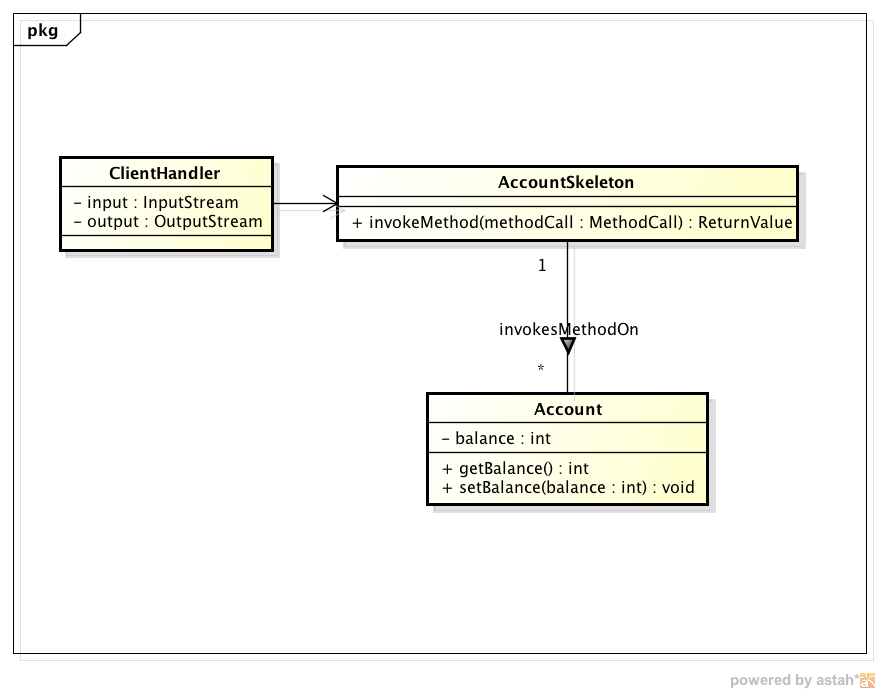
\includegraphics[scale = 0.5]{images_objectcaching/rmiServerImpl}  
  \caption{RMI-Serverimplementation Domain Class Diagramm}
  \label{fig:rmiserverimpl}
\end{figure}

\subsubsection{Schnittstelle zum Framework}
\label{sec:schn-zum-fram}

Damit diese Clienthandler-Objekte mit den
richtigen Skeleton-Objekte initialisiert werden, bietet das System
eine zentrale ServerSystem-Klasse. Das Framework erzeugt eine Instanz
der ServerSystem-Klasse. Wenn sich Client mit dem Server verbindet,
fordert das Framework von diese Serversystem\-instanz einen
Clienthandler an. Dieser wird mit den richtigen SkeletonObjekte
initialisiert. Das Framework übergibt dem Clienthandler die Input- und OutputStreamobjekte.

\section{Concurrency Control Implementierung }
\label{sec:conc-contr-impl}

Das System soll Lost Updates verhindern, indem Optimistic Concurrency
eingesetzt wird. Das heisst, bei Schreibzugriffen wird überprüft, ob die Daten zwischenzeitlich verändert wurden. Dazu
versioniert der Server die Objekte, deren Methoden auf entfernten
Clients aufgerufen werden können. Die Versionen werden in der HashMap
$W$ gespeichert. Die HashMap $W$ verwendet als Key die ID der Objekte
und als Value die Version. Bei jedem Schreibzugriff, das heisst bei
einem \verb|setBalance()|, der ohne Konflikt ausgeführt wird, wird die
Version des Objektes inkrementiert. Zusätzlich merkt sich der Server
für jeden Client und für jedes Objekt, auf welcher Version des
Objektes zuletzt ein Lesezugriff (\verb|getBalance()|) stattgefunden hat. Dafür
wird eine zweite HashMap $R$ verwendet. In der HashMap $R$ wird als Key
ein String verwendet, der sich aus der IP-Adresse und der
Objekt-ID des Methodenaufrufs zusammensetzt. Als Value speichert die HashMap $R$ die Version ab.
Ruft ein Client
\verb|getBalance()| auf, holt der Server die aktuelle Version aus dem
der HashMap $W$ und speichert sie in mit der entsprechenden IP und
Objekt-ID in der HashMap $R$ ab.

Ruft ein Client \verb|setBalance()| auf, prüft der Server, ob die
Version des Clients aus der HashMap $R$ tiefer ist, als die aktuelle
Version aus der HashMap $W$. Ist dies der Fall, wird der Methodenaufruf
abgebrochen und der Client erhält eine Nachricht, dass die Methode
nicht ausgeführt werden konnte.
